% Presentación: modelo y linealización del robot PIR
% (capítulo CapModelosDinamicos, sección "Robot de tipo péndulo invertido
% sobre ruedas"). Código: ../STM32_code/USER/control_lqr_mode{0,1,2,3}.jl
% (diseño LQR en Julia) y ../STM32_code/APP/app_control.c (firmware).
% Compilar con: pdflatex presentacion_PIR.tex
\documentclass[10pt,aspectratio=169]{beamer}
\usetheme[progressbar=frametitle,numbering=fraction]{metropolis}

\usepackage[spanish,es-noshorthands]{babel}
\usepackage[utf8]{inputenc}
\usepackage[T1]{fontenc}
\usepackage{lmodern}
\usepackage{amsmath,amssymb}
\usepackage{siunitx}
\usepackage{booktabs}

\graphicspath{{../figuras/}{figuras/}}   % figuras/: generadas con figuras_control.jl

% Colores del libro (preambulo/estilo_colores.tex)
\definecolor{azullibro}{HTML}{1D477B}
\definecolor{rojolibro}{HTML}{C4161D}
\definecolor{celeste}{HTML}{D9F3FD}
\setbeamercolor{frametitle}{bg=azullibro,fg=white}
\setbeamercolor{progress bar}{fg=rojolibro,bg=celeste}
\setbeamercolor{alerted text}{fg=rojolibro}
\setbeamercolor{block title}{bg=azullibro!15,fg=azullibro}
\setbeamercolor{block body}{bg=azullibro!5}

% Notación
\newcommand{\tS}{\tau_\Sigma}           % tau_i + tau_d
\newcommand{\tD}{\tau_\Delta}           % tau_i - tau_d (giro positivo hacia la derecha)
\newcommand{\sth}{\sin\theta_c}
\newcommand{\cth}{\cos\theta_c}
\newcommand{\vx}{\mathbf{x}}
\newcommand{\vu}{\mathbf{u}}
\newcommand{\vz}{\mathbf{z}}
\newcommand{\vy}{\mathbf{y}}
\newcommand{\vr}{\mathbf{r}}
\newcommand{\gr}[1]{\textcolor{gray!45}{#1}}  % entrada eliminada del modelo
\newcommand{\rf}{\text{ref}}
% Ecuación resaltada (sin barra de título)
\newcommand{\resaltar}[1]{\begin{center}\colorbox{celeste}{$\displaystyle #1$}\end{center}}

\title{Robot de tipo péndulo invertido sobre ruedas (PIR)}
\subtitle{Modelo no lineal y linealización para el diseño LQR}
\date{}

\begin{document}

\maketitle

%--------------------------------------------------------------------
\begin{frame}{El robot PIR y sus variables}
\begin{columns}[c]
\column{0.42\textwidth}
\centering
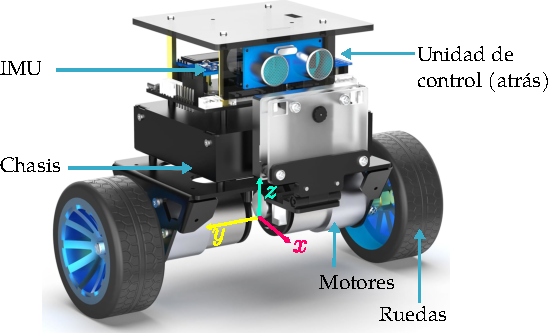
\includegraphics[width=\linewidth]{robot_render.pdf}

\column{0.56\textwidth}
\small
\textbf{Estado} (6 variables):
\[
\vx=\begin{bmatrix} x & v & \theta_c & \omega_c & \delta & \omega_\delta\end{bmatrix}^{\!\top}
\]
\vspace{-1em}
\begin{itemize}
  \item $x,\,v$: avance y velocidad del punto $O$
  \item $\theta_c,\,\omega_c$: inclinación (cabeceo) del cuerpo
  \item $\delta,\,\omega_\delta$: giro (guiñada) del robot, positivo hacia la
  derecha (horario visto desde arriba)
\end{itemize}
\textbf{Entradas:} torques de los motores, $\vu=\begin{bmatrix}\tau_i & \tau_d\end{bmatrix}^{\!\top}$

\medskip
\textbf{Hipótesis:} ruedas idénticas que no deslizan, $v_k=r\,\omega_k$.

\medskip
\alert{Inestable en lazo abierto:} hay que actuar sobre las ruedas para no caer.
\end{columns}
\end{frame}

%--------------------------------------------------------------------
\begin{frame}{1. Rueda}
\begin{columns}[c]
\column{0.3\textwidth}
\centering
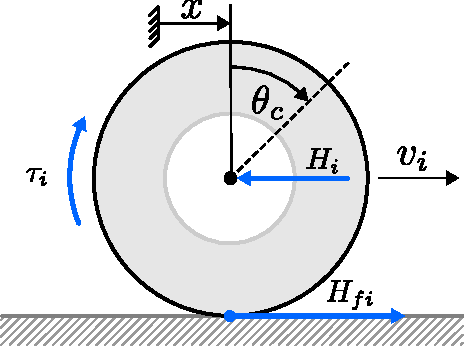
\includegraphics[width=\linewidth]{modelo_rueda.pdf}

\column{0.68\textwidth}
Para la rueda $k\in\{i,d\}$, con fricción $H_{fk}$ y reacción del cuerpo $H_k$:
\begin{align*}
  \text{traslación:}\quad & m\,\dot v_k = H_{fk}-H_k\\
  \text{rotación:}\quad   & J_r\,\dot\omega_k = \tau_k - r\,H_{fk}
\end{align*}
Se elimina $H_{fk}$ y se usa $\dot\omega_k=\dot v_k/r$ (sin deslizamiento):
\resaltar{\Big(m+\frac{J_r}{r^2}\Big)\dot v_k=\frac{\tau_k}{r}-H_k,\qquad k\in\{i,d\}}
La inercia de la rueda aparece como  $J_r/r^2$.
\end{columns}
\end{frame}

%--------------------------------------------------------------------
\begin{frame}{2. Avance e inclinación}
\begin{columns}[c]
\column{0.36\textwidth}
\centering
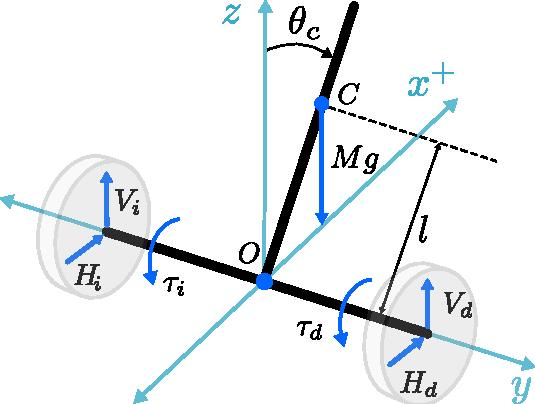
\includegraphics[width=\linewidth]{modelo_avance.pdf}

\small $\tS=\tau_i+\tau_d$,\quad $v=\dfrac{v_i+v_d}{2}$

\column{0.62\textwidth}
\small
Newton sobre el cuerpo (centro de masa $C$ a distancia $l$ de $O$):
\begin{align*}
  H_i+H_d &= M\,\tfrac{d^2}{dt^2}\big(x+l\sth\big)\\
  V_i+V_d-Mg &= M\,\tfrac{d^2}{dt^2}\big(l\cth\big)\\
  J_c\,\ddot\theta_c &= (V_i+V_d)\,l\sth-(H_i+H_d)\,l\cth-\tS
\end{align*}
Combinadas con la suma de las ecuaciones de las ruedas:
\resaltar{\begin{aligned}
  Q_2\,\dot v + Ml\cth\,\dot\omega_c &= \frac{\tS}{r} + Ml\,\omega_c^2\sth\\
  Ml\cth\,\dot v + Q_1\,\dot\omega_c &= Mgl\sth - \tS
\end{aligned}}
$Q_1=J_c+Ml^2$,\qquad $Q_2=M+2m+2J_r/r^2$
\end{columns}
\end{frame}

%--------------------------------------------------------------------
\begin{frame}{3. Giro}
\begin{columns}[c]
\column{0.32\textwidth}
\centering
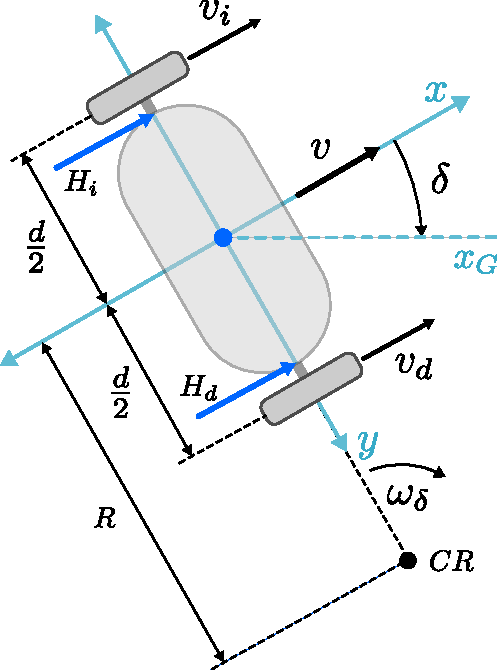
\includegraphics[width=\linewidth]{modelo_direccion.pdf}

\small $\tD=\tau_i-\tau_d$

\column{0.66\textwidth}
$\delta$ es positivo hacia la derecha (horario visto desde arriba): la rueda
izquierda más rápida hace crecer $\delta$.
\begin{align*}
  \text{dinámica:}\quad & J_\delta\,\ddot\delta=\frac{d}{2}\,(H_i-H_d)\\
  \text{cinemática:}\quad & \omega_\delta=\frac{v_i-v_d}{d}
\end{align*}
Restando las ecuaciones de las ruedas y eliminando $H_i-H_d$:
\resaltar{Q_3\,\dot\omega_\delta=\frac{\tD}{r},\qquad
  Q_3=md+\frac{d\,J_r}{r^2}+\frac{2J_\delta}{d}}
El giro queda \alert{desacoplado} del avance y de la inclinación,
y ya es lineal.
\end{columns}
\end{frame}

%--------------------------------------------------------------------
\begin{frame}{Modelo no lineal}
Al resolver el sistema $2\times2$ en $(\dot v,\dot\omega_c)$, con
$\Delta(\theta_c)=Q_1Q_2-M^2l^2\cos^2\theta_c$:
\begin{align*}
  \dot x &= v\\
  \dot v &= \frac{\big(\tfrac{Q_1}{r}+Ml\cth\big)\tS-M^2l^2g\sth\cth+Q_1Ml\,\omega_c^2\sth}{\Delta(\theta_c)}\\
  \dot\theta_c &= \omega_c\\
  \dot\omega_c &= \frac{MglQ_2\sth-\big(Q_2+\tfrac{Ml}{r}\cth\big)\tS-M^2l^2\,\omega_c^2\sth\cth}{\Delta(\theta_c)}\\
  \dot\delta &= \omega_\delta\\
  \dot\omega_\delta &= \frac{\tD}{r\,Q_3}
\end{align*}
\end{frame}

%--------------------------------------------------------------------
\begin{frame}{Linealización}
\textbf{Equilibrio} (vertical y en reposo):\quad
$\bar\theta_c=\bar v=\bar\omega_c=\bar\omega_\delta=0,\ \ \bar\tau_i=\bar\tau_d=0$;\quad
$\bar x,\ \bar\delta$ arbitrarios.

\medskip
\textbf{Jacobianos:}\
$A=\partial f/\partial \vx\,\big|_{\text{eq}}$,\
$B=\partial f/\partial \vu\,\big|_{\text{eq}}$.
Equivale a conservar solo los términos de primer orden:
\[
  \sin\theta_c\approx\theta_c,\qquad \cos\theta_c\approx1,\qquad
  \omega_c^2\approx 0,\qquad \tS\sth\approx0
\]
El denominador se evalúa en el equilibrio:
\resaltar{\Delta_0=\Delta(0)=Q_1Q_2-M^2l^2
  = J_cM+\big(J_c+Ml^2\big)\Big(2m+\frac{2J_r}{r^2}\Big)}
\begin{align*}
  \dot v &\approx \frac{-M^2l^2g\,\theta_c+\big(\tfrac{Q_1}{r}+Ml\big)\tS}{\Delta_0},&
  \dot\omega_c &\approx \frac{MglQ_2\,\theta_c-\big(Q_2+\tfrac{Ml}{r}\big)\tS}{\Delta_0}
\end{align*}
\end{frame}

%--------------------------------------------------------------------
\begin{frame}{Modelo lineal \texorpdfstring{$\dot\vx=A\vx+B\vu$}{dx/dt = Ax + Bu}}
\[
\underbrace{\begin{bmatrix}\dot x\\ \dot v\\ \dot\theta_c\\ \dot\omega_c\\ \dot\delta\\ \dot\omega_\delta\end{bmatrix}}_{\dot\vx}
=\underbrace{\begin{bmatrix}
0&1&0&0&0&0\\
0&0&a_{23}&0&0&0\\
0&0&0&1&0&0\\
0&0&a_{43}&0&0&0\\
0&0&0&0&0&1\\
0&0&0&0&0&0
\end{bmatrix}}_{A}
\underbrace{\begin{bmatrix}x\\ v\\ \theta_c\\ \omega_c\\ \delta\\ \omega_\delta\end{bmatrix}}_{\vx}
+\underbrace{\begin{bmatrix}
0&0\\ b_{2}&b_{2}\\ 0&0\\ b_{4}&b_{4}\\ 0&0\\ b_{6}& -b_{6}
\end{bmatrix}}_{B}
\underbrace{\begin{bmatrix}\tau_i\\ \tau_d\end{bmatrix}}_{\vu}
\]
\[
  a_{23}=-\frac{M^2l^2g}{\Delta_0},\quad
  a_{43}=\frac{MglQ_2}{\Delta_0},\qquad
  b_{2}=\frac{Q_1+Mlr}{r\,\Delta_0},\quad
  b_{4}=-\frac{Q_2+\frac{Ml}{r}}{\Delta_0},\quad
  b_{6}=\frac{1}{r\,Q_3}
\]
\begin{itemize}\small
  \item $(x,v,\theta_c,\omega_c)$: subsistema de avance--inclinación, excitado por $\tS$.
  \item $(\delta,\omega_\delta)$: doble integrador de giro, excitado por $\tD$.
\end{itemize}
\end{frame}

%--------------------------------------------------------------------
\begin{frame}{Del modelo al código (Julia y firmware)}
\begin{columns}[t]
\column{0.36\textwidth}
\small
\begin{tabular}[t]{@{}ll@{}}
\toprule
Modelo & \texttt{control\_lqr\_modeN.jl}\\
\midrule
$J_r$ & \texttt{inercia}\\
$J_c$ & \texttt{J\_centroide}\\
$J_\delta$ & \texttt{J\_Y\_delta}\\
$l$ & \texttt{L}\\
$\Delta_0$ & \texttt{Q\_aux}\\
$a_{23},\,a_{43}$ & \texttt{A\_23}, \texttt{A\_43}\\
$b_2,\,b_4$ & \texttt{B\_21}, \texttt{B\_41}\\
$b_6$ & \texttt{B\_61}\\
\bottomrule
\end{tabular}

\column{0.62\textwidth}
\small
\textbf{Escala de la entrada.} El código usa
$\vu=\dfrac{r}{J_r}\begin{bmatrix}\tau_i&\tau_d\end{bmatrix}^{\!\top}$
(\si{\meter\per\second\squared}; columna~1: motor izquierdo, columna~2: derecho):
\[
  B_{\text{código}}=\frac{J_r}{r}\,B
\]
\textbf{Sentido del giro:} el mismo de la figura en Julia y en el firmware,
$\delta$ positivo hacia la \alert{derecha}. Por eso \texttt{B\_61}~$=b_6>0$
(motor izquierdo) y \texttt{B\_62}~$=-b_6$. El firmware mide
\[
  \omega_\delta=\frac{v_i-v_d}{d}\ (\texttt{gyro\_z}),\qquad
  \delta=\int\omega_\delta\,dt\ (\texttt{angle\_z}),
\]
y las referencias son \texttt{ref\_yaw}~$=\delta_\rf$ y
\texttt{ref\_wd}~$=\omega_{\delta,\rf}$.
\end{columns}
\end{frame}

%--------------------------------------------------------------------
\begin{frame}{Valores numéricos}
\small
Con los parámetros del fabricante del robot
($m=\SI{35}{\gram}$, $r=\SI{33.6}{\milli\meter}$, $M=\SI{1.07}{\kilo\gram}$,
$l=\SI{38.3}{\milli\meter}$, $d=\SI{161.2}{\milli\meter}$):
\[
A\approx\begin{bmatrix}
0&1&0&0&0&0\\
0&0&-14.62&0&0&0\\
0&0&0&1&0&0\\
0&0&419.1&0&0&0\\
0&0&0&0&0&1\\
0&0&0&0&0&0
\end{bmatrix},
\qquad
B_{\text{código}}\approx\begin{bmatrix}
0&0\\ 0.0585&0.0585\\ 0&0\\ -1.251&-1.251\\ 0&0\\ 0.940&-0.940
\end{bmatrix}
\]
\textbf{Polos en lazo abierto:}\quad
$s=0\ (\times4),\qquad s=\pm\sqrt{a_{43}}\approx\pm\SI{20.5}{\radian\per\second}$

\medskip
\alert{El polo en $+20.5$ hace inestable al péndulo:} se necesita
realimentación de estado, $\vu=-K\vx$, con $K$ calculada por LQR
(modo~0 del firmware, \texttt{control\_lqr\_mode0.jl}: $\vu=-K(\vx-\vx_\rf)$ con
\texttt{ref\_pos} y \texttt{ref\_yaw}).
\end{frame}

%====================================================================
% Control de velocidades con el modelo lineal
% (figuras de figuras/ generadas con figuras_control.jl)
%====================================================================
\begin{frame}{Velocidad lineal: modelo reducido}
\small
\textbf{Objetivo:} que $v$ siga a $v_\rf$; la posición $x$ no interesa.
Su columna en $A$ es nula: ningún estado depende de $x$ y $\dot x=v$ solo
integra la velocidad $\Rightarrow$ \alert{se elimina solo $x$}.
\begin{columns}[c]
\column{0.31\textwidth}
\footnotesize\renewcommand{\arraystretch}{0.85}
\[
A=\begin{bmatrix}
\gr0&\gr1&\gr0&\gr0&\gr0&\gr0\\
\gr0&0&a_{23}&0&0&0\\
\gr0&0&0&1&0&0\\
\gr0&0&a_{43}&0&0&0\\
\gr0&0&0&0&0&1\\
\gr0&0&0&0&0&0
\end{bmatrix}
\]
\column{0.67\textwidth}
\footnotesize\renewcommand{\arraystretch}{0.85}
\resaltar{\vx_v=\begin{bmatrix}v\\ \theta_c\\ \omega_c\\ \delta\\ \omega_\delta\end{bmatrix},\quad
  \dot\vx_v=\underbrace{\begin{bmatrix}0&a_{23}&0&0&0\\0&0&1&0&0\\0&a_{43}&0&0&0\\
    0&0&0&0&1\\0&0&0&0&0\end{bmatrix}}_{A_v}\vx_v
  +\underbrace{\begin{bmatrix}b_2&b_2\\0&0\\b_4&b_4\\0&0\\b_6&-b_6\end{bmatrix}}_{B_v}
  \begin{bmatrix}\tau_i\\ \tau_d\end{bmatrix}}
\end{columns}
\begin{itemize}
  \item Se conservan el giro y \textbf{las dos entradas}: un solo LQR,
  $\vu=-K\,(\vx_v-\vx_\rf)$, con
  $\vx_\rf=\begin{bmatrix}v_\rf&0&0&\delta_\rf&0\end{bmatrix}^{\!\top}$,
  $K\in\mathbb{R}^{2\times5}$, $Q\in\mathbb{R}^{5\times5}$, $R\in\mathbb{R}^{2\times2}$.
  \item \textbf{Polos:} $s=0$ (de $v$), $\pm\sqrt{a_{43}}\approx\pm20.5$ y $0$ doble
  (de $\delta$). Sin fricción, todo $\bar v$ constante es equilibrio con
  $\theta_c=0$ y $\vu=0$.
  \item \textbf{Controlable} con los dos motores (rango 5). Con uno solo el rango
  cae a 4: el modo en $s=0$ de $v$ y el de $\delta$ no se pueden fijar por
  separado.
\end{itemize}
\end{frame}

%--------------------------------------------------------------------
\begin{frame}{Velocidad de giro: modelo reducido}
\small
\textbf{Objetivo:} que $\omega_\delta$ siga a $\omega_{\delta,\rf}$; la orientación
$\delta$ no interesa. Su columna en $A$ es nula: ningún estado depende de $\delta$ y
$\dot\delta=\omega_\delta$ solo integra la velocidad de giro
$\Rightarrow$ \alert{se elimina solo $\delta$}.
\begin{columns}[c]
\column{0.31\textwidth}
\footnotesize\renewcommand{\arraystretch}{0.85}
\[
A=\begin{bmatrix}
0&1&0&0&\gr0&0\\
0&0&a_{23}&0&\gr0&0\\
0&0&0&1&\gr0&0\\
0&0&a_{43}&0&\gr0&0\\
\gr0&\gr0&\gr0&\gr0&\gr0&\gr1\\
0&0&0&0&\gr0&0
\end{bmatrix}
\]
\column{0.67\textwidth}
\footnotesize\renewcommand{\arraystretch}{0.85}
\resaltar{\vx_\omega=\begin{bmatrix}x\\ v\\ \theta_c\\ \omega_c\\ \omega_\delta\end{bmatrix},\quad
  \dot\vx_\omega=\underbrace{\begin{bmatrix}0&1&0&0&0\\0&0&a_{23}&0&0\\0&0&0&1&0\\
    0&0&a_{43}&0&0\\0&0&0&0&0\end{bmatrix}}_{A_\omega}\vx_\omega
  +\underbrace{\begin{bmatrix}0&0\\b_2&b_2\\0&0\\b_4&b_4\\b_6&-b_6\end{bmatrix}}_{B_\omega}
  \begin{bmatrix}\tau_i\\ \tau_d\end{bmatrix}}
\end{columns}
\begin{itemize}
  \item Se conservan el avance y \textbf{las dos entradas}: un solo LQR,
  $\vu=-K\,(\vx_\omega-\vx_\rf)$, con
  $\vx_\rf=\begin{bmatrix} x_\rf&0&0&0&\omega_{\delta,\rf}\end{bmatrix}^{\!\top}$,
  $K\in\mathbb{R}^{2\times5}$, $Q\in\mathbb{R}^{5\times5}$, $R\in\mathbb{R}^{2\times2}$.
  \item \textbf{Polos:} $0$ doble (de $x$), $\pm\sqrt{a_{43}}\approx\pm20.5$ y $0$
  (de $\omega_\delta$). Sin fricción, todo $\bar\omega_\delta$ constante es equilibrio
  con $\vu=0$: el robot gira en el sitio, en $x=x_\rf$.
  \item \textbf{Controlable} con los dos motores (rango 5). Con uno solo el rango
  cae a 4, como en la velocidad lineal.
\end{itemize}
\end{frame}

%--------------------------------------------------------------------
\begin{frame}{Velocidad lineal y velocidad de giro: modelo reducido}
\small
\textbf{Objetivo:} que $v$ siga a $v_\rf$ y $\omega_\delta$ a $\omega_{\delta,\rf}$;
no interesan $x$ ni $\delta$. Sus columnas en $A$ son nulas: ningún estado depende
de ellas $\Rightarrow$ \alert{se eliminan $x$ y $\delta$}.
\begin{columns}[c]
\column{0.31\textwidth}
\footnotesize\renewcommand{\arraystretch}{0.85}
\[
A=\begin{bmatrix}
\gr0&\gr1&\gr0&\gr0&\gr0&\gr0\\
\gr0&0&a_{23}&0&\gr0&0\\
\gr0&0&0&1&\gr0&0\\
\gr0&0&a_{43}&0&\gr0&0\\
\gr0&\gr0&\gr0&\gr0&\gr0&\gr1\\
\gr0&0&0&0&\gr0&0
\end{bmatrix}
\]
\column{0.67\textwidth}
\footnotesize\renewcommand{\arraystretch}{0.85}
\resaltar{\vx_{v\omega}=\begin{bmatrix}v\\ \theta_c\\ \omega_c\\ \omega_\delta\end{bmatrix},\quad
  \dot\vx_{v\omega}=\underbrace{\begin{bmatrix}0&a_{23}&0&0\\0&0&1&0\\
    0&a_{43}&0&0\\0&0&0&0\end{bmatrix}}_{A_{v\omega}}\vx_{v\omega}
  +\underbrace{\begin{bmatrix}b_2&b_2\\0&0\\b_4&b_4\\b_6&-b_6\end{bmatrix}}_{B_{v\omega}}
  \begin{bmatrix}\tau_i\\ \tau_d\end{bmatrix}}
\end{columns}
\begin{itemize}
  \item Un solo LQR con \textbf{las dos entradas}: $\vu=-K\,(\vx_{v\omega}-\vx_\rf)$, con
  $\vx_\rf=\begin{bmatrix}v_\rf&0&0&\omega_{\delta,\rf}\end{bmatrix}^{\!\top}$,
  $K\in\mathbb{R}^{2\times4}$, $Q\in\mathbb{R}^{4\times4}$, $R\in\mathbb{R}^{2\times2}$.
  \item \textbf{Polos:} $0$ (de $v$), $\pm\sqrt{a_{43}}\approx\pm20.5$ y $0$
  (de $\omega_\delta$). Todo par $(\bar v,\bar\omega_\delta)$ constante es equilibrio
  con $\vu=0$: el robot recorre una circunferencia de radio $\bar v/\bar\omega_\delta$.
  \item \textbf{Controlable} con los dos motores (rango 4); con uno solo, rango 3.
  \item Con $Q$ diagonal y $R=\rho I$, $K$ sale \alert{desacoplada}: mismas
  ganancias de avance en los dos motores; la de $\omega_\delta$, con signo opuesto.
\end{itemize}
\end{frame}

%====================================================================
% Acción integral con realimentación de estado
% (presentación "Acción Integral Variables De Estado")
%====================================================================
\begin{frame}{Acción integral con realimentación de estado}
\small
Con $\vu=K_r\vr-K\vx$, la salida llega a la referencia solo si $A$, $B$ y $C$ se
conocen \alert{exactamente y no hay perturbaciones (fricción, diferencia en motores \dots)}.
Se agrega un integrador por cada salida que debe seguir una referencia:
\[
  \dot\vz=\vr-\vy,\qquad \vy=C\vx,\qquad
  \vu=K_r\,\vr-K\vx-K_i\,\vz
\]
\textbf{Diseño:} con el sistema aumentado en $\begin{bmatrix}\vx&\vz\end{bmatrix}^{\!\top}$,
\resaltar{\begin{bmatrix}\dot\vx\\ \dot\vz\end{bmatrix}
  =\underbrace{\begin{bmatrix}A&0\\-C&0\end{bmatrix}}_{A^*}
   \begin{bmatrix}\vx\\ \vz\end{bmatrix}
  +\underbrace{\begin{bmatrix}B\\0\end{bmatrix}}_{B^*}\vu
  +\begin{bmatrix}0\\ I\end{bmatrix}\vr,
  \qquad
  \begin{bmatrix}K&K_i\end{bmatrix}=\text{LQR}\big(A^*,B^*,Q^*,R\big)}
\begin{itemize}
  \item En el equilibrio $\dot\vz=0\Rightarrow\vy=\vr$: el estado $\vz$ se
  \alert{autoajusta}, aun con errores de modelo o perturbaciones constantes.

\end{itemize}
\end{frame}

%--------------------------------------------------------------------
\begin{frame}{Velocidad lineal con acción integral (modo 1)}
\small
Salida con integrador: $y=v$, $r=v_\rf$, con el modelo reducido de velocidad lineal
(sin $x$).
\begin{columns}[c]
\column{0.30\textwidth}
\footnotesize
\[
  \vx_v=\begin{bmatrix}v\\ \theta_c\\ \omega_c\\ \delta\\ \omega_\delta\end{bmatrix}
\]
\[
  C_v=\begin{bmatrix}1&0&0&0&0\end{bmatrix}
\]
\[
  \dot z_v=v_\rf-C_v\vx_v
\]
\column{0.68\textwidth}
\footnotesize\renewcommand{\arraystretch}{0.85}\setlength{\arraycolsep}{3pt}
\resaltar{\begin{bmatrix}\dot\vx_v\\ \dot z_v\end{bmatrix}
  =\underbrace{\left[\begin{array}{ccccc|c}
    0&a_{23}&0&0&0&0\\
    0&0&1&0&0&0\\
    0&a_{43}&0&0&0&0\\
    0&0&0&0&1&0\\
    0&0&0&0&0&0\\ \hline
    -1&0&0&0&0&0
  \end{array}\right]}_{A_v^*}
  \begin{bmatrix}\vx_v\\ z_v\end{bmatrix}
  +\underbrace{\left[\begin{array}{cc}
    b_2&b_2\\0&0\\b_4&b_4\\0&0\\b_6&-b_6\\ \hline 0&0
  \end{array}\right]}_{B_v^*}
  \begin{bmatrix}\tau_i\\ \tau_d\end{bmatrix}
  +\begin{bmatrix}0\\ 1\end{bmatrix}v_\rf}
\end{columns}
\begin{itemize}
  \item $\vu=-K\,(\vx_v-\vx_\rf)-K_i\,z_v$, con
  $\vx_\rf=\begin{bmatrix}0&0&0&\delta_\rf&0\end{bmatrix}^{\!\top}$: $v_\rf$ entra
  solo por el integrador, como en el firmware ($K\,v$, no $K\,(v-v_\rf)$). $K\in\mathbb{R}^{2\times5}$,
  $K_i\in\mathbb{R}^{2\times1}$, por LQR sobre $(A_v^*,B_v^*)$ con
  $Q^*\in\mathbb{R}^{6\times6}$, $R\in\mathbb{R}^{2\times2}$.
  \item $(A_v^*,B_v^*)$ es \textbf{controlable} (rango 6).
  \item En el equilibrio $v=v_\rf$ \alert{exactamente}, aun con fricción o pendiente.
  El rumbo $\delta$ solo se regula con $K$: si la perturbación afecta distinto a los
  dos motores, puede quedar un error en $\delta$.
\end{itemize}
\end{frame}

%--------------------------------------------------------------------
\begin{frame}{Velocidad de giro con acción integral (modo 2)}
\small
Salida con integrador: $y=\omega_\delta$, $r=\omega_{\delta,\rf}$, con el modelo
reducido de velocidad de giro (sin $\delta$).
\begin{columns}[c]
\column{0.30\textwidth}
\footnotesize
\[
  \vx_\omega=\begin{bmatrix}x\\ v\\ \theta_c\\ \omega_c\\ \omega_\delta\end{bmatrix}
\]
\[
  C_\omega=\begin{bmatrix}0&0&0&0&1\end{bmatrix}
\]
\[
  \dot z_\omega=\omega_{\delta,\rf}-C_\omega\vx_\omega
\]
\column{0.68\textwidth}
\footnotesize\renewcommand{\arraystretch}{0.85}\setlength{\arraycolsep}{3pt}
\resaltar{\begin{bmatrix}\dot\vx_\omega\\ \dot z_\omega\end{bmatrix}
  =\underbrace{\left[\begin{array}{ccccc|c}
    0&1&0&0&0&0\\
    0&0&a_{23}&0&0&0\\
    0&0&0&1&0&0\\
    0&0&a_{43}&0&0&0\\
    0&0&0&0&0&0\\ \hline
    0&0&0&0&-1&0
  \end{array}\right]}_{A_\omega^*}
  \begin{bmatrix}\vx_\omega\\ z_\omega\end{bmatrix}
  +\underbrace{\left[\begin{array}{cc}
    0&0\\b_2&b_2\\0&0\\b_4&b_4\\b_6&-b_6\\ \hline 0&0
  \end{array}\right]}_{B_\omega^*}
  \begin{bmatrix}\tau_i\\ \tau_d\end{bmatrix}
  +\begin{bmatrix}0\\ 1\end{bmatrix}\omega_{\delta,\rf}}
\end{columns}
\begin{itemize}
  \item $\vu=-K\,(\vx_\omega-\vx_\rf)-K_i\,z_\omega$, con
  $\vx_\rf=\begin{bmatrix}x_\rf&0&0&0&\omega_{\delta,\rf}\end{bmatrix}^{\!\top}$ (la ley
  del modelo reducido más el término integral), $K\in\mathbb{R}^{2\times5}$,
  $K_i\in\mathbb{R}^{2\times1}$, por LQR sobre $(A_\omega^*,B_\omega^*)$ con
  $Q^*\in\mathbb{R}^{6\times6}$, $R\in\mathbb{R}^{2\times2}$.
  \item $(A_\omega^*,B_\omega^*)$ es \textbf{controlable} (rango 6).
  \item En el equilibrio $\omega_\delta=\omega_{\delta,\rf}$ \alert{exactamente}. La
  posición $x$ solo se regula con $K$: con fricción o pendiente el robot puede quedar
  desplazado de $x_\rf$ mientras gira.
\end{itemize}
\end{frame}

%--------------------------------------------------------------------
\begin{frame}{Velocidad lineal y de giro con acción integral (modo 3)}
\small
Salidas con integrador:
$\vy=\begin{bmatrix}v&\omega_\delta\end{bmatrix}^{\!\top}$,
$\vr=\begin{bmatrix}v_\rf&\omega_{\delta,\rf}\end{bmatrix}^{\!\top}$,
$\vz=\begin{bmatrix}z_v&z_\omega\end{bmatrix}^{\!\top}$.
\begin{columns}[c]
\column{0.30\textwidth}
\footnotesize
\[
  \vx_{v\omega}=\begin{bmatrix}v\\ \theta_c\\ \omega_c\\ \omega_\delta\end{bmatrix}
\]
\[
  C_{v\omega}=\begin{bmatrix}1&0&0&0\\0&0&0&1\end{bmatrix}
\]
\[
  \dot\vz=\vr-C_{v\omega}\vx_{v\omega}
\]
\column{0.68\textwidth}
\footnotesize\renewcommand{\arraystretch}{0.85}\setlength{\arraycolsep}{3pt}
\resaltar{\begin{bmatrix}\dot\vx_{v\omega}\\ \dot\vz\end{bmatrix}
  =\underbrace{\left[\begin{array}{cccc|cc}
    0&a_{23}&0&0&0&0\\
    0&0&1&0&0&0\\
    0&a_{43}&0&0&0&0\\
    0&0&0&0&0&0\\ \hline
    -1&0&0&0&0&0\\
    0&0&0&-1&0&0
  \end{array}\right]}_{A_{v\omega}^*}
  \begin{bmatrix}\vx_{v\omega}\\ \vz\end{bmatrix}
  +\underbrace{\left[\begin{array}{cc}
    b_2&b_2\\0&0\\b_4&b_4\\b_6&-b_6\\ \hline 0&0\\0&0
  \end{array}\right]}_{B_{v\omega}^*}
  \begin{bmatrix}\tau_i\\ \tau_d\end{bmatrix}
  +\begin{bmatrix}0\\ I\end{bmatrix}\vr}
\end{columns}
\begin{itemize}
  \item $\vu=-K\,(\vx_{v\omega}-\vx_\rf)-K_i\vz$, con
  $\vx_\rf=\begin{bmatrix}0&0&0&\omega_{\delta,\rf}\end{bmatrix}^{\!\top}$ ($v_\rf$ entra
  solo por el integrador), $K\in\mathbb{R}^{2\times4}$, $K_i\in\mathbb{R}^{2\times2}$,
  por LQR sobre $(A_{v\omega}^*,B_{v\omega}^*)$ con $Q^*\in\mathbb{R}^{6\times6}$,
  $R\in\mathbb{R}^{2\times2}$.
  \item $(A_{v\omega}^*,B_{v\omega}^*)$ es \textbf{controlable} (rango 6).
  \item En el equilibrio $v=v_\rf$ y $\omega_\delta=\omega_{\delta,\rf}$ exactamente: el
  radio de la trayectoria, $v_\rf/\omega_{\delta,\rf}$, no depende de la fricción.
\end{itemize}
\end{frame}

%--------------------------------------------------------------------
\begin{frame}{Simulación e implementación digital}
\small
\textbf{Simulación:} lazo cerrado en $\begin{bmatrix}\vx&\vz\end{bmatrix}^{\!\top}$,
\[
  \begin{bmatrix}\dot\vx\\ \dot\vz\end{bmatrix}
  =\begin{bmatrix}A-BK&-BK_i\\-C&0\end{bmatrix}
   \begin{bmatrix}\vx\\ \vz\end{bmatrix}
  +\begin{bmatrix}BK_r\\ I\end{bmatrix}\vr,\qquad
  \vy=\begin{bmatrix}C&0\end{bmatrix}\begin{bmatrix}\vx\\ \vz\end{bmatrix}
\]
\textbf{Implementación:} con tiempo de muestreo $T_s$ (en el firmware
$T_s=\SI{5}{\milli\second}$, \SI{200}{\hertz}), el integrador se aproxima con
$\dot\vz\approx\dfrac{\vz[n+1]-\vz[n]}{T_s}$. En cada periodo:
\begin{columns}[c]
\column{0.44\textwidth}
\resaltar{\begin{aligned}
  \mathbf{e}[n]&=\vr[n]-\vy[n]\\
  \vu[n]&=-\big(K\vx[n]+K_i\vz[n]\big)+K_r\vr[n]\\
  \vz[n+1]&=\vz[n]+T_s\,\mathbf{e}[n]
\end{aligned}}
\column{0.54\textwidth}
\footnotesize
\begin{tabular}{@{}lllll@{}}
\toprule
Caso & Modo & $\vy$ (integradas) & $K$ & $K_i$\\
\midrule
Velocidad lineal & 1 & $v$ & $2\times5$ & $2\times1$\\
Velocidad de giro & 2 & $\omega_\delta$ & $2\times5$ & $2\times1$\\
Lineal y de giro & 3 & $v,\ \omega_\delta$ & $2\times4$ & $2\times2$\\
\bottomrule
\end{tabular}
\end{columns}
\medskip
$K_r$ puede dejarse en $0$: el integrador garantiza $\vy=\vr$ en estado estacionario.
En el firmware $K_r\vr=K\vx_\rf$: $v_\rf$ entra solo por el integrador y
$\omega_{\delta,\rf}$ también por el error $\omega_\delta-\omega_{\delta,\rf}$.
\end{frame}

%--------------------------------------------------------------------
\begin{frame}{Modos de control en el firmware}
\small
Cada modo tiene su diseño en Julia (\texttt{USER/control\_lqr\_modeN.jl}), que escribe
\texttt{lqr\_gain\_modeN.h}; \texttt{app\_control.c} compila los cuatro y en todos
$\begin{bmatrix}K&K_i\end{bmatrix}$ es de $2\times6$.

\footnotesize
\begin{tabular}{@{}cllll@{}}
\toprule
Modo & Controla & Estado realimentado & Integradores & Referencias\\
\midrule
0 & posición y rumbo & $x,\,v,\,\theta_c,\,\omega_c,\,\delta,\,\omega_\delta$ & --- & \texttt{ref\_pos}, \texttt{ref\_yaw}\\
1 & velocidad lineal & $v,\,\theta_c,\,\omega_c,\,\delta,\,\omega_\delta$ & $z_v$ & \texttt{ref\_vel}, \texttt{ref\_yaw}\\
2 & velocidad de giro & $x,\,v,\,\theta_c,\,\omega_c,\,\omega_\delta$ & $z_\omega$ & \texttt{ref\_pos}, \texttt{ref\_wd}\\
3 & velocidad lineal y de giro & $v,\,\theta_c,\,\omega_c,\,\omega_\delta$ & $z_v,\,z_\omega$ & \texttt{ref\_vel}, \texttt{ref\_wd}\\
\bottomrule
\end{tabular}
\small
\begin{itemize}\setlength{\itemsep}{1pt}
  \item \textbf{Medición} cada \SI{5}{\milli\second}: $v$, $\omega_\delta$ (y por integración
  $x$, $\delta$) de los encoders; $\theta_c$ del filtro de Kalman de la IMU, medido
  respecto al equilibrio real $\theta_0=\SI{0.0349}{\radian}$; $\omega_c$ por diferencia
  finita de $\theta_c$.

  \item \textbf{Arranque:} al activarse el control el robot pasa \SI{5}{\second} en el
  modo~0 y luego cambia al modo programado (\texttt{LQR\_MODE}); en ejecución se cambia con
  \texttt{Set\_Control\_Mode()}.
\end{itemize}
\end{frame}

%--------------------------------------------------------------------



\end{document}
